\Cref{fig:main} shows the main empirical story. In panel (a), the unconstrained edge ansatz carries many more parameters yet generalizes worse than the $D_4$-equivariant edge model. At 600 training examples, edge/none reaches about $0.63$ test accuracy while edge/$D_4$ reaches about $0.69$ with a smaller train-test gap. This reproduces the central lesson of Meyer et al.: the correct board symmetry removes irrelevant functions from the hypothesis class rather than simply shrinking the model.

Panel (b) makes the picture less binary. Full $D_4$ is the conservative default, but $C_4$ tracks it closely across the data grid: it is slightly ahead at 30 examples, and from 120 through 600 examples the two stay essentially together while weaker or unconstrained sharing lags. We read this cautiously. It does not establish that partial symmetry is generally better; it shows that symmetry strength is a tunable bias, with rotation-only equivariance preserving most of the benefit while relaxing reflection constraints. The random-sharing control in \cref{fig:controls}(a) is the guardrail: it fixes parameter count but scrambles the group-orbit structure, and performs substantially worse than orbit-based sharing at every subgroup. The useful prior is the board geometry, not just the smaller circuit.

The strongest effect, in \cref{fig:main}(c), comes from enriching the symmetry rather than weakening it. The original edge/$D_4$ model sits near $0.69$; adding both winning-line channels to the same equivariant circuit lifts the best $D_4$ model to roughly $0.80$, with the $C_4$ variant close behind. This is the central result: the gain comes not from abandoning symmetry, but from giving the equivariant ansatz direct access to the motifs that decide the label.

\Cref{fig:controls} rules out two simpler explanations. The gain is not arbitrary parameter reduction, since matched-size random sharing falls short of orbit sharing in panel (a). It is not simply more parameters either: edge+lines/$D_4$ has 90 parameters, more than edge/$D_4$ at 54 but far below the 204 of the unshared baseline. Panel (c) makes the point geometric: accuracy does not follow parameter count, and edge+lines models occupy a higher band at modest size. The ablation in panel (b) confirms the composition: line-only circuits help, but the strongest model combines local edge structure with both winning-line channels.

\begin{figure*}[t]
\centering
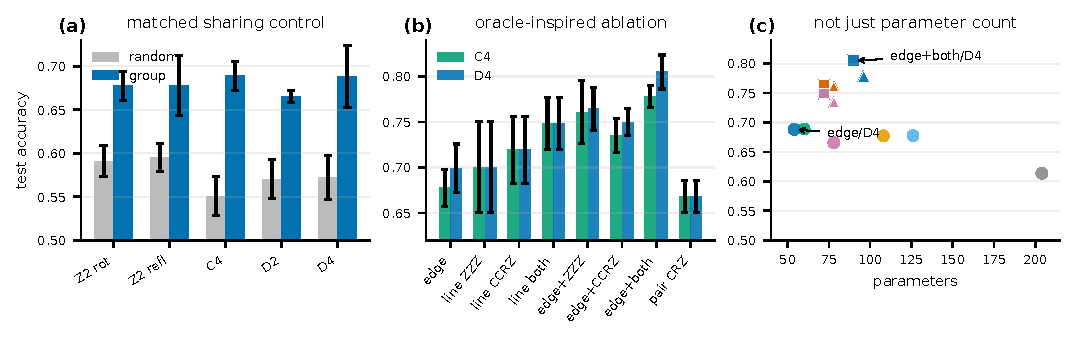
\includegraphics[width=.94\textwidth]{gfx/fig3_controls}
\caption{\normalsize Controls and ablations. (a) Parameter-matched random sharing underperforms group-orbit sharing. (b) Ablations are anchored by the labelled original edge/$D_4$ ansatz; the strongest model combines edge interactions with both line channels. (c) Accuracy is not explained by parameter count alone.}
\label{fig:controls}
\end{figure*}
